\chapter{Implementing device-independent quantum key distribution}

\section{Platform comparison}

DIQKD security protocols relies on entanglement to generate a provably secure key.
Key rates, asserting the amount of secure key bit that can be extracted per experiment rounds, is the reference benchmark to compare suggestions of potential DIQKD implementations.
As the key rates presented in Sec.~\ref{sec:Pavel} and Sec.~\ref{sec:Brown} are recent and were not easily exploitable at the time of preparing this thesis, we here focus on key rates based on the CHSH score to compare DIQKD implementations.

\medbreak

In order to implement DIQKD, a first requirement is to be able to entrust all assumptions made on the protocol.
Specifically, the no-leakage assumption need particular attention.
For a Bell test, no information about the input of a party should influence the outcome of the other party's measurement.
This locality loophole is often closed by using a space-like separation of Alice and Bob's lab, see e.g. \cite{Hensen2015,Giustina2015,Shalm2015}.
When it comes to DIQKD, this is however more complex as not only the inputs but also the outcomes of each rounds have to be kept secret.
Therefore, proposal of a DIQKD experiment have to address this loophole by suggesting a relevant way to isolate Alice and Bob's lab.

\medbreak

CHSH based key rates increase with the CHSH score.
Subsequently, proposed DIQKD experiments should be based on a plateform known to be able to generate highly entangled state leading to high CHSH score in a loophole-free manner.

\medbreak

A critical factor in implementing DIQKD is the ability for the experiment to operate at a high repetition rate.
Firstly, the generated key is intended for use with symmetric cryptography protocol such as the XOR cipher, which require a bit of key per bit to encrypt.
Additionally, a fast repetition rate enables the experiment to tolerate more loss, i.e. maintaining a practical key generation rate per second even for a lower CHSH score.

\medbreak

In the rest of this section, we will examine two common platforms for implementing DIQKD: one utilizing heralded entanglement and the other based on purely photonic circuits. 
We will provide a brief overview of the advantages and disadvantages of each approach.

\subsection{Heralded entanglement}

The objective of heralded entanglement experiments is to generate a strong entanglement between two quantum systems, held by Alice and Bob.
Such quantum systems can be of different nature, and notably include NV-center, single atoms in cavities and trapped ions.
A particularity of these systems is that they are capable of emitting photons that are entangled with the inner state of the system.
Therefore, by sending these photons to a central station that performs Bell-state measurements, Alice and Bob can entangle their quantum system through a process known as \textit{entanglement swapping}.

Combining the capability of creating highly entangled state with high detection efficiencies, high \acrshort{chsh} score can be achieve with heralding experiments. 
Such experiments have thus been successfully use to perform loophole-free Bell experiments~\cite{Hensen2015,Rosenfeld2017}.
Importantly for DIQKD, heralded entanglement systems are scalable by nature as the transmission loss is managed thanks to the heralding process.

On the downside, heralded entanglement realizations run at a low repetition rate. 
This is mainly due to resetting the system between measurements.
Furthermore, this approach requires heavy machineries which can not easily be embedded or minimized to work in data centers or on satellites as desired for industrial DIQKD applications.
As such, while heralded entanglement systems are a great tool for proof-of-concept experiments, they may not be the ideal candidate for long-term applications.

\medbreak

A first DIQKD experiment, making use of trapped ions, has been reported in ~\cite{Nadlinger2022}.
This was made possible from the strong entanglement between two ions separated by $2\mathrm{m}$, yielding a high CHSH score of $S\approx 2.677$ and having a low quantum bit error rate of $Q\approx 0.0144$
Including finite-size effects, this experiment achieved key rate of $r \approx 0.0639$.
Coupled with a possible repetition of rate $\approx120\mathrm{Hz}$, and a reported rate of $61\mathrm{Hz}$, it took $7.9\mathrm{h}$ to generate a key of $95\,884$ bits.
Following this first realization, another demonstration of DIQKD using trapped ions has extended the distance between parties by two order of magnitude~\cite{Zhang2022}.

\subsection{Photonic setups}

The thoroughly studied photonic setups can produce photons which are entangled in some degree-of-freedom.
If the common approach uses photons entangled in polarization, there is other possibilities such as path-entangled single-photon~\cite{Caspar2020}.
Leveraging the entanglement production capabilities of these setups, experimental loophole-free Bell tests have been successfully conducted~\cite{Giustina2015,Shalm2015,Li2018}.

Photonic setups offer numerous advantage over the heralded entanglement approach.
Firstly, they provide a high repetition rate which can be order of magnitude higher than what has been achieved with trapped ions.
Additionally, on a more long term aspect, the photonic platform has a promising potential for commercial applications, mainly thanks to integrated photonic circuits which enable the implementation of complex circuits that can be embedded on a chip.
In fact, photonic device-dependent QKD realization has been performed with system embedded on satellite~\cite{Liao2017}, and rack unit for data centers are already commercially available~\cite{Pljonkin2018}. 

For the implementation of DIQKD protocols, photonic setups have two main limitations.
First, photonic sources used in most Bell test demonstrations produce states which are far from ideal two-qubit states, resulting in a low CHSH score.
For example, photon entangled in polarization, generated by a SPDC source can only achieve a CHSH score of $S\approx 2.35$~\cite{Vivoli2015b}.
Furthermore, photonic implementations are highly susceptible to losses, mainly from distribution in optical fiber and from non-resolution in single-photon detectors.
This leads to low CHSH score and a challenging scalability with respect to longer transmission distances.
However, these limitations can be mitigated.
Recent theoretical advances in DIQKD protocols coupled with more efficient quantum optical devices can lead to possible photonic DIQKD realizations.
Furthermore, quantum repeater could help transmitting photons over long distances without breaking entanglement~\cite{Sangouard2011}.

\medbreak

Photonic setups are hence a natural candidate for DIQKD experiments and more long-term applications~\cite{Zapatero2023}.
Encouragingly, a first proof-of-concept realization of DIQKD with photons entangled in polarization has been reported~\cite{Liu2022}.
This experiment is, however, not complete, as random basis switching has been omitted.

\medbreak

More efforts are therefore needed in order to see a photonic DIQKD realization. 
Complementary to protocol improvements we detailed in Chap.~\ref{chap:entropybound}, it also worth exploring new photonic experiment designs.
In the next section, we present a common approach to photonic DIQKD, based on photons entangled in polarization.
The key rate obtained with this setup is used as a benchmark to newly suggested experiment design.
Then, in the last section of this chapter, we show how photonic experiments can be design in an automated manner, as we proposed in Article 4.
Applied to DIQKD, this lead to new setups which are promising candidates for photonic DIQKD implementations.


\section{DIQKD with polarization-entangled photons}
\label{sec:PolarizationDIQKD}

A standard approach to implement DIQKD with photons is to use polarization entangled photons generated by a spontaneous down-conversion source (SPDC) and measured in different polarization basis thanks to wave plates, polarization beam-splitters and single-photon detectors.
This typical setup, sometimes referred called the \textit{SPDC setup}, is depicted in \reffig{spdc}.
This approach is the one chosen in the proof-of-concept experiment \cite{Liu2022} and is often used to benchmark theoretical key rate improvements~\cite{Ho2020,Sekatski2021}.

\begin{figure}[t]
	\begin{center}
		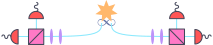
\includegraphics[width=0.95\textwidth]{chapters/deviceindependent/img/spdc.pdf}
	\end{center}
	\caption{SPDC setup. A SPDC source (yellow star) sends photons entangled in polarization (blue lines), with one part send to Alice and one send to Bob.
	Locally, each party dispose of wave plates (purple ellipse) used to chose the measurement basis according to the measurement setting. This is followed by a polarising beamsplitter (pink sliced square) with each of the two outputs measured by NPNR detectors.}
	\label{fig:spdc}
\end{figure}

\medbreak

Let us briefly described the statistics obtained from this implementation.
An SPDC source is often implemented as a laser pulsed into a non-linear crystal.
This emits photons in coupled modes, with mode $a$ send to Alice and mode $b$ send to Bob.
Note that here we only consider a single mode, whereas, in practice, multiple modes can be created.
We denote $a,a_\perp$ the two orthogonal polarizations of Alice's mode, and, similarly $b,b_\perp$ for Bob.
The state emitted is given by
\begin{equation}
	\ket{\psi} = \sqrt{1-T_g}\sqrt{1-T_{g'}}\exp(T_{g} a^\dag\,a^\dag_\perp - T_{g'}b^\dag\,b_\perp^\dag)\ket{00}
\end{equation}
with $T_g = \tanh(g)$ and $T_{g'} = \tanh(g')$, and where $g$ and $g'$ are the squeezing parameters given by the non-linear susceptibility of the crystal and by the power of the pump.

For each measurement input, Alice rotates her measurement basis with mean of wave plates.
Formally, for angles $(\alpha_x,\phi_x)$ corresponding to the input choice $x$, the two orthogonal polarization change following
\begin{equation}
	\begin{split}
		a &= \cos(\alpha_x)\tilde{a} + e^{i\phi_x}\sin(\alpha_x)\tilde{a}_\perp, \\
		a_\perp &= e^{-i\phi_x}\sin(\alpha_x)\tilde{a}-\cos(\alpha_x)\tilde{a}_\perp.
	\end{split}
\end{equation}
where $(\tilde{a},\tilde{a}_\perp)$ form a new polarization basis.
Similarly, Bob obtains a new polarization basis $(\tilde{b},\tilde{b}_\perp)$ from angles $(\beta_y,\varphi_y)$ for input $y$.

Finally, each polarizing beam-splitter outputs two-modes, on for each polarization basis, that are measured using single-photon detectors.
For Alice, the detectors will measure the modes $\tilde{a},\tilde{a}_\perp$, respectively, while for Bob they will resolve $\tilde{b}$ for one and $\tilde{b}_\perp$ for the other.
Such detectors are \acrfull{NPNR} detectors with outcomes $+1$, or \textit{click}, when a photonic signal is detected and $-1$, or \textit{no-click}, otherwise.
These detector have an efficiency $\eta$, i.e. in the presence of photons the outcome should be $+1$ with probability $\eta$.
Formally, a $\eta$-efficient NPNR detector on a mode $\tilde{a}$, is characterized by the POVM $\{M_{-1}^{\tilde{a}},1-M_{+1}^{\tilde{a}}\}$ where
\begin{equation}
	M_{-1}^{\tilde{a}} = (1-\eta)^{\tilde{a}^\dag\tilde{a}}.
\end{equation}
To obtain binary outcomes, Alice and Bob bin their four potential outcomes $\{p_H,p_V\}=\{\pm1,\pm1\}$.
For the outcomes pair $\{p_H,p_V\}$, a clever binning choice gives the outcome
\begin{equation}
	p=\begin{cases}
		+1, &\text{ if } \{p_H,p_V\}=\{+1,-1\}\\
		-1, &\text{otherwise}.
	\end{cases}
\end{equation}

Combing the expression of the state, the measurement basis choices and the detection operators, one can compute the statistics $p(ab|xy)$ as a function of the squeezing parameters, Alice and Bob measurements angles and detector efficiencies.
The full derivation of these statistics can be found in \cite{Vivoli2015b} and \cite{Ho2020}.

\medbreak

\begin{figure}[ht!]
	\begin{center}
		\includegraphics[width=.95\textwidth]{chapters/deviceindependent/img/key_rate_spdc.pdf}
	\end{center}
	\caption{Key rate with efficiency. The blue line correspond to the key rate obtained from a SPDC setup when all source and measurement parameters are optimized. The bump is an artifact due to a more precise optimisation performed for efficiency close the critical one. The orange curve gives the key rate obtained for two-qubit partially entangled state, as a reference.}
	\label{fig:SPDC_kr}
\end{figure}

The statistics computed from the SPDC setup allow to study its application for DIQKD.
This is achieved by optimising the key rate over the squeezing parameters and measurement angles.
With this method, we can recover the critical detection efficiency by repeating the optimisation for progressively smaller efficiency $\eta$ until no positive key rate is obtained.
Note that this possible as losses in the optical fiber before detection can be reformulate as inefficient NPRP detectors, i.e. these two types of losses commute. 
The evolution of the key rate with the detection efficiency is shown in \reffig{SPDC_kr}.

Using the key rate \refeq{Ho}, with fine-grained error correction and noisy preprocessing, the mono-mode SPDC setup have a key rate of $r\approx 0.2552$ for the ideal case $\eta=1$. 
When allowing for more modes, the key rate goes up to $\approx 0.295$.
This setup also requires a detection efficiency of at least $\eta\approx 0.826$ to yield a positive key rate.
This critical efficiency is independent on the amount of modes we consider as a difference in CHSH violation between single and multi-mode SPDC source is only noticeable for efficiency higher that $0.9$~\cite{Vivoli2015b}.


%Give key rates from Melvyn's paper.
%
%Also key rate are equivalent to two-qubit partially entangled state when considering better key rate (generalized CHSH).

\section{Automatic design of photonic experiments}

If photonic setups are a promising plateform for quantum information processing and, in particular, for DIQKD, finding a suitable photonic experiment design is cumbersome.
Indeed, thanks to integrated photonic~\cite{Pelucchi2021} there is the possibility to implement complex circuits, combining numerous optical devices.
Therefore, a systematic search through all possible implementations seems unrealistic.
Furthermore, for each photonic setup, carrying the computation either by hand is a time-consuming task while using numerical analysis based on available Fock-representation framework quickly turn resource heavy when precise computation and more optical modes are considered.
Finally, with a constant evolution of DIQKD protocols, new implementations need to be proposed continuously.

To circumvent these issues, in Article 4~\cite{Valcarce2022b}, we propose an approach using machine learning and an efficient custom-made photonic simulation framework which, together, can propose photonic design matching a given figure of merit, e.g. a DIQKD key rate. 
In the next two subsections, we give an overview of this method.
Then, we show how our method performs for the design of DIQKD experiments as well as for another figure of merit.

\begin{figure}
	\begin{center}
		\includegraphics[width=0.95\textwidth]{chapters/deviceindependent/img/illustration_automated_design.png}
	\end{center}
	\caption{Artist's impression of the automated design of photonic experiments. \textcopyright\, Dowinson Nguyen.}
	\label{fig:}
\end{figure}



\subsection{Simulating quantum optical circuits}

Photonic circuits can be seen as a quantum circuits where each mode $i$ is a bosonic mode characterized by the bosonic operators $a_i,a_i^\dagger$, and where gates are transformations of these modes.
We restrict ourselves to optical transformation that are commonly available in quantum optics laboratory : single- and two-modes squeezers, displacements, phase-shifters and beam-splitters.
To measure these bosonic modes, we focus on non photon-number resolving (NPNR) detectors sometimes called single-photon detectors, which have outcome $+1$ or \textit{click}, when a signal is detected and $-1$, or \textit{no-click}, otherwise.
In addition to these operations, we also include heralding operations, conditioning the state of the circuit on the presence of signal in the heralded mode.


In order to efficiently explore these photonic setups, there is the need for a fast and accurate simulation framework.
Therefore, we based our approach on the Gaussian representation of state and operations, allowing for an exact and memory-efficient representation of circuits.
We then developed a numerical framework using this representation to efficiently evaluate any given photonic circuit.


\paragraph{Gaussian Quantum optics}

Consider a $n$-mode bosonic system. 
Each mode $i$ can be described in term of quadrature operators; the position $x_i=(a_i^\dagger+a_i)/2$ and the momentum $p_i=i(a_i^\dagger-a_i)/2$ operator.
The entire circuit is thus characterized by the vector $\mathbf{q}=(q_1,\dots,q_{2n})=(x_1,p_1,\dots,x_n,p_n)$.

Gaussian states, such as the vacuum state, are fully characterized by a displacement vector $\mathbf{\mu}$ and a covariance matrix $\Sigma$.
Elements of these two object are functions of $\mathbf{q}$, they are given by
\begin{align}
	\mathbf{\mu} = (\mu_1,\dots,\mu_{2n}), \qquad &\text{with}\quad \mu_i = \mean{q_i} = \trr{\rho q_i} \\
	\Sigma = \begin{pmatrix} \Sigma_{11} & \dots & \Sigma_{1,2n} \\
							\vdots & \ddots & \vdots \\
						\Sigma{2n,1} & \dots & \Sigma_{2n,2n}\end{pmatrix} , \qquad &\text{with}\quad \Sigma_{i,j} = \frac{\mean{q_i q_j + q_j q_i}}{2}-\mu_i \mu_j.
\end{align}
This representation is compact as it only need $2n(n+1)$ real parameters to fully characterized a $n$-mode bosonic system.

Gaussian transformations are transformations which conserve the Gaussian properties of Gaussian states. 
The optical devices listed above are all Gaussian transformations.
Such transformation are represented by a vector $\mathbf{d}$ of size $2n$ and by a symplectic matrix $M$ of size $2n\times2n$.
Apply on a Gaussian state $(\mathbf{\mu},\Sigma)$, such transformations output
\begin{equation}
	(\mathbf{\mu},\sigma)\; \mapsto\; (M\mathbf{\mu} + d,\, M\Sigma M^T).
\end{equation}

The no-click probability of a NPNR detector with efficiency $\eta$, on mode $i$, $p_{\circ,i}$, is computed from the displacement vector and covariance matrix of a Gaussian state following
\begin{equation}
p_{\circ i} =\frac{2}{2-\eta}\sqrt{\frac{(\det \Sigma)^{-1}}{ \det(\Sigma^{-1}+F)}}
e^{-\frac{1}{2}{\mathbf{\mu} }^T\left( \Sigma^{-1} - \Sigma^{-1} (\Sigma^{-1}+F)^{-1} \Sigma^{-1} \right){\mathbf{\mu} }}
\end{equation}
where
\begin{equation}
F= \left(\begin{array}{cc}
    \frac{4\eta}{2-\eta} & 0 \\
    0 & \frac{4\eta}{2-\eta}
    \end{array}\right)_{2i-1,2i} \oplus 0_{2n-2}.
\end{equation}
Trivially, the click probability in mode $i$ is given by $p_{\bullet,i}=1-p_{\circ,i}$.

Heralded operations are non-Gaussian operations.
However, the state $\rho_{\bullet,i}$resulting of a $n$-mode Gaussian state conditioned on a click in a mode $i$, can be expressed as a sum of two $(n-1)$-modes Gaussian state
\begin{equation}
    \rho_{\bullet,i} = \frac{\rho_{\lnot,i} - p_{\circ,i} \rho_{\circ,i}}{1 - p_{\circ,i}}
\end{equation}
where $\rho_{\lnot,i}$ is the Gaussian state with the mode $i$ traced out and where $\rho_{\circ,i}$ is the Gaussian state after a no-click event.
Therefore, with $2^{n-m}(2m^2+3m+1)$ real parameters, we can represent a $n$-mode photonic circuits undergoing $n-m$ heralding operations.

More details on the exact expression of the Gaussian transformation for each optical devices, on the expression used to obtain the statistics of joined NPNR detections, and their derivations can be found in Appendix A of Article 4.

\paragraph{QuantumOpticalCircuits.jl}

Using the Julia programming language~\cite{Bezanson2017}, we developed \textsc{QuantumOpticalCircuits.jl}, a package to simulate efficiently and accurately photonic setups~\cite{Valcarce2021}.
This package relies on the Gaussian representation to store states in a compact form and to compute accurately the effect of optical gates and the outcomes of single photon detectors.
It includes all the optical devices we listed above as well as NPNR detectors and heralded operations.

Our package makes extensive use of the multiple-dispatch paradigm of the Julia programming language.
Hence, it can easily be extended to include other operations or measurements.
Furthermore, we design this package with ease-of-use in mind, so that programming a photonic setup to be simulated becomes accessible.
Finally, even if it is less efficient, we also provide a Fock representation back-end, as this representation is more common in the community.
A simple example using this framework can be seen in \reffig{QOC.jl}.

\begin{figure}
	\begin{center}
		\includegraphics[width=1\textwidth]{chapters/deviceindependent/img/quantumopticalcircuits.png}
	\end{center}
	\caption{Example usage of QuantumOpticalCircuits.jl in the Julia REPL. }
	\label{fig:QOC.jl}
\end{figure}


\subsection{Reinforcement Learning}

\acrfull{rl} is a machine learning paradigm that involves an intelligent agent learning to perform a task by interacting with an environment~\cite{Sutton2018}.
Schematically, from the current state of an environment, an agent will chose an action to be performed.
Feedback is then provided in the form of the new state of the environment and a \textit{reward}, designed to quantify the quality of the action-state pair with respect to the goal task.
From this feedback, the agent updates the way actions are chosen in order to maximize the reward received. 

One of the key advantage of \acrshort{rl} is that is does not require pre-generated data to be trained on, unlike supervised and unsupervised learning.
This is particularly beneficial when generating data is costly as it is the case with the simulation of optical circuits.

\medbreak

\acrshort{rl} has seen numerous successful applications to a great variety of tasks, from learning to play games~\cite{Mnih2015,Silver2017,Vinyals2019} to finding new algorithm for matrix multiplications~\cite{Fawzi2022}.
In the field of quantum physics, \acrshort{rl} has been applied to design quantum error correction algorithms~\cite{Andreasson2019,Nautrup2019,Sweke2020}, quantum gates~\cite{Niu2019}, or new quantum experiments~\cite{Melnikov2018,Krenn2016,Krenn2020,Krenn2021}, in particular to design photonic Bell test experiments~\cite{Melnikov2020}.

Motivated by these past works, in Article 4, we proposed an approach that combine reinforcement learning and our photonic circuit simulation framework to generate new photonic experiment designs.
As an agent we use \acrfull{ppo}, a deep reinforcement learning algorithm, known to be sample efficient~\cite{Schulman2017}.
Actions that can be chosen from are optical devices that act on a specific mode or pair of modes.
After appending a chosen action to the photonic circuit, an optimization over the optical devices' parameters is run in order to maximize a given function of the statistics, e.g. a DIQKD key rate, from which the reward is computed.
From past experiences -- state, chosen action, new state and reward -- the \acrshort{ppo} algorithm updates its policy so that future chosen actions maximize the reward obtained.


\subsection{Application to DIQKD}

We applied our automated approach to the design of DIQKD experiments.
We limit ourselves to 3-modes photonic circuits with the third one being heralded before Alice and Bob's measurements.
The measurements we consider are heterodyne measurements, i.e. a displacement operation followed by a NPNR detector.

First, we picked a reward to maximize the key rate ~\refeq{Ho} achieved in an ideal scenario, i.e. in the absence of losses and noises.
After training a \acrshort{ppo} agent on that task, we obtained a fairly complex photonic circuit, composed of 12 elements.
In the ideal case, this setup achieve a key rate of $r_{Ho}\approx 0.914$, outperforming the benchmark implementation detailed in \ref{sec:PolarizationDIQKD}.
However, this setup seems not so robust to losses as we were able to obtain positive key rate for $\eta \apprge 0.874$ only.
Then, we crafted a reward to maximize the robustness of the key rate to losses.
Our method provided a simple circuit of only 7 optical devices, more robust that the reference implementation.
Indeed, this setup output key rate $r_{Ho}\geq10^{-8}$ for efficiency $\apprge 0.8245$. 
Furthermore, the obtained key rate are consistently higher that the one achieved by the benchmark setup.
These setups as well as their key rate with efficiency can be found in Article 4.


\subsection{Application toward continuous-variable DIQKD}

Our automated approach for designing photonic experiments can be readily extended to implement any task that can be expressed as a function of measurements.
An interesting task for quantum cryptography is \textit{continuous-variable} DIQKD; DIQKD implementations in which Alice and Bob perform homodyne measurements, resolving the quadratures $x,p$ of bosonic modes.
These measurements are particularly relevant as they are known to be robust to losses and can be performed at a high repetition rate.
However, if a violation of the CHSH inequality -- the first step toward DIQKD -- can be obtained in this regime, the implementation with the highest violation that has been proposed so far yield a score of $S \approx 2.046$~\cite{GarciaPatron2004,GarciaPatron2005}.
From this low violation current DIQKD protocols provide a mere positive key rates, e.g. even considering the unrealistic case of $H(A_0'|B_2)=0.0$, \refeq{Ho} gives only $r_{Ho}\approx 10^{-2}$.
To improve on this violation, a proposal combing homodyne and NPNR detectors has shown an expected violation of $S\approx 2.25$~\cite{Cavalcanti2011}.
Another proposal has shown that a Bell violation of $S \approx 2.35$ can be obtained provided that one trust the measurement devices, which is not-relevant for DIQKD~\cite{Thearle2018}.

It is in this context that we apply our automated method with the task of maximizing the CHSH violation using solely homodyne measurement, heralding operations, and the optical devices listed above.
We limit our selves to the measurement settings proposed in \cite{GarciaPatron2005} and to a sign binning of the homodyne measurement outcome.
After learning, our intelligent agent proposed the circuit depicted in \reffig{homodyne}. 
Interestingly, this circuit attain a CHSH score of $S\approx 2.068$. 
Encouragingly, this score is closed to $2.072$, the maximum violation that could be reached with homodyne measurements, sign binning and any state of the form $\ket{\psi}=\sum_i c_i \ket{i,i}$~\cite{Munro1999}.

\begin{figure}[ht]
	\begin{center}
		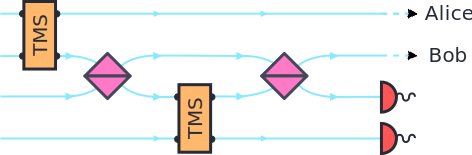
\includegraphics[width=0.95\textwidth]{chapters/deviceindependent/img/homodyne.pdf}
	\end{center}
	\caption{Circuit achieving a CHSH score $S\approx 2.068$. The blue lines are bosonic modes. The yellow rectangle labeled TMS represent two-mode squeezer, with optimal squeezing parameters $g_1=0.44689$ and $g_2=8.47\times 10^{-3}$ respectively. The two sliced pink squares are beam-splitters with optimal parameters $\theta_1 = 0.04202$ and $\theta_2 = 0.04338$. The two red half circles represent NPNR dectors heralding the modes 3 and 4. The final prepared state is post-selected on a double click, i.e. in
	both mode 3 and 4, which occurs with a probability of $p\approx 4.05\times10^{-7}$. The first mode is then send to Alice while the second is send to Bob.}
	\label{fig:homodyne}
\end{figure}


